\documentclass{beamer}
\usepackage{beamerthemesplit}
\usetheme{SPbGU}
%{CambridgeUS}
% Выпишем часть возможных стилей, некоторые из них могут содержать
% дополнительные опции
% Darmstadt, Ilmenau, CambridgeUS, default, Bergen, Madrid, AnnArbor,Pittsburg, Rochester,
% Antiles, Montpellier, Berkley, Berlin
\usepackage{pdfpages}
\usepackage{amsmath}
\usepackage{cmap} % for serchable pdf's
\usepackage[T2A]{fontenc} 
\usepackage[utf8]{inputenc}
\usepackage[english,russian]{babel}
\usepackage{indentfirst}
\usepackage{amsmath}
\usepackage{dot2texi}
\usepackage{tikz}
\usepackage{fancyvrb}
\usepackage{graphicx}
\usepackage{array}
%\usepackage{animate}
\usepackage{multimedia}
%\usepackage[usenames,dvipsnames]{color}
\usetikzlibrary{shapes,arrows}
% Если у вас есть логотип вашей кафедры, факультета или университета, то
% его можно включить в презентацию.

%\usefoottemplate{\vbox{}}%  \tinycolouredline{structure!25}% {\color{white}\textbf{\insertshortauthor\hfill% \insertshortinstitute}}% \tinycolouredline{structure}% {\color{white}\textbf{\insertshorttitle}\hfill}% }}

%\logo{
\includegraphics[width=1cm]{SPbGU_Logo.png}}

\title[]{Лексический анализ динамически формируемых строковых выражений}
\institute[СПбГУ]{
Санкт-Петербургский государственный университет \\
Математико-Механический факультет \\
Кафедра системного программирования }

\author[Полубелова Марина]{Полубелова Марина Игоревна, 444 гр. \\
  \and  
  {\bfseries Научный руководитель:} ст.преп. Григорьев С.В. \\ 
  \and  
  {\bfseries Рецензент:} \small{программист OOO ``ИнтеллиДжей Лабс''} Беляков~А.М. \\ 
}

\date{15 июня 2015г.}

\begin{document}
{
\begin{frame}
    \begin{center}
        {
\includegraphics[width=1cm]{SPbGU_Logo.png}}
    \end{center}
    \titlepage
\end{frame}
}

\definecolor{green}{RGB}{0, 100, 0}
\definecolor{orange}{RGB}{255,110,0}
\definecolor{gray}{RGB}{105,105,105}
\begin{frame}[fragile]
\transwipe[direction=90]
\frametitle{Примеры}
\begin{itemize}

\item Встроенный SQL в С\#
\begin{Verbatim}[commandchars=\\\{\}]
\textcolor{green}{private void} \textcolor{blue}{Go} (\textcolor{blue}{int} cond)\{
	\textcolor{blue}{string} columnName = cond > \textcolor{gray}{3} ? \textcolor{red}{"X"}:(cond < \textcolor{gray}{0} ? \textcolor{red}{"Y"}:\textcolor{red}{"Z"});
	\textcolor{blue}{string} queryString = 
	             \textcolor{red}{"SELECT name"} + columnName + \textcolor{red}{" FROM table"};
	Program.ExecuteImmediate(queryString);
\}
\end{Verbatim}
		
\item Динамически генерируемый HTML в PHP-программах
\begin{Verbatim}[commandchars=\\\{\}]	
<?php 
    \$name = \textcolor{red}{'your name'};
    echo \textcolor{red}{'<table>} 
         \textcolor{red}{<tr><th>Name</th></tr>}  
         \textcolor{red}{<tr><td>'}.\$name.\textcolor{red}{'</td></tr>} 
         \textcolor{red}{</table>'};
?>
\end{Verbatim}
\end{itemize}
\end{frame}

\begin{frame}
\transwipe[direction=90]
\frametitle{Область применения}
\begin{itemize}
\item Реинжиниринг программного обеспечения
	\begin{itemize}
	\item Анализ и трансформация систем, использующие строковые выражения
	\end{itemize}
\item Поддержка строковых выражений в IDE
	\begin{itemize}
    \item Статический поиск ошибок
	\item Подсветка синтаксиса
	\item Рефакторинги
	\end{itemize}
\end{itemize}
\end{frame}

\begin{frame}[fragile]
\transwipe[direction=90]
\frametitle{Существующие подходы}
Проверка корректности программ, получающихся в результате использования строковых выражений:
\begin{itemize}
	\item Проверка включения языков
	\item Проведение лексического анализа и синтаксического разбора компактного представления множества динамически формируемых строковых выражений
\end{itemize}	
\end{frame}


\begin{frame}
\transwipe[direction=90]
\frametitle{Обзор существующих решений и аналогов}
\begin{itemize}
\item Java String Analyzer
	\begin{itemize}
	\item регулярная аппроксимация строкового выражения
	%\item проверка включения языков
	\end{itemize}
	
\item PHP String Analyzer 
	\begin{itemize}
	\item контексно-свободная аппроксимация строкового выражения
	%\item проверка включения языков
	\end{itemize}
	
\item Alvor 
	\begin{itemize}
	%\item плагин к Eclipse для проверки встроенного в Java SQL
	\item нет поддержки строковых операций, за исключением конкатенации, и циклов
	%\item лексический анализ проводится отдельно от синтаксического разбора
	\end{itemize}

\item Алгоритм абстрактного синтаксичеcкого анализа Kyung-Goo Doh, Hyunha Kim, David A. Schmidt

\item Курсовые работы Вербицкой Екатерины, Полубеловой Марины
\end{itemize}
\end{frame}


\begin{frame}[fragile]
\transwipe[direction=90]
\frametitle{Постановка задачи}

\textbf{Цель}: реализация инструмента для проведения лексического анализа динамически формируемых строковых выражений

\begin{itemize}
\item Реализовать механизм для лексического анализа выражений, формируемых с помощью циклов и строковых операций%, сохраняющий привязку частей динамически формируемого строкового выражения к исходному коду и привязку лексических единиц внутри каждой части
\item Сохранить привязку лексических единиц к исходному коду
\item Реализовать генератор лексических анализаторов
\end{itemize}

\end{frame}

\begin{frame}
\transwipe[direction=90]
\frametitle{Лексический анализ строковых выражений}
\begin{itemize}
\item На вход анализатору подается конечный автомат, полученный в результате аппроксимации строкового выражения
\item На выходе получаем либо конечный автомат над токенами, либо список лексических ошибок. Токен содержит в себе:
	\begin{itemize}
	\item идентификатор токена
	\item конечный автомат --- часть множества значений строкового выражения, которая выделена лексическим анализатором в данный тип токена
	\end{itemize}
\end{itemize}

\begin{block}{}
\textbf{Задача лексического анализа}: получение конечного автомата над токенами из конечного автомата над символами
\end{block}

\end{frame}

\begin{frame}[fragile]
\transwipe[direction=90]
\frametitle{Пример}
\begin{itemize}
\item 
\begin{Verbatim}[commandchars=\\\{\}]
\textcolor{green}{private void} \textcolor{blue}{Go} (\textcolor{blue}{int} cond)\{
	\textcolor{blue}{string} columnName = cond > \textcolor{gray}{3} ? \textcolor{red}{"X"}:(cond < \textcolor{gray}{0} ? \textcolor{red}{"Y"}:\textcolor{red}{"Z"});
	\textcolor{blue}{string} queryString = 
	             \textcolor{red}{"SELECT name"} + columnName + \textcolor{red}{" FROM table"};
	Program.ExecuteImmediate(queryString);
\}
\end{Verbatim}
		
\item Результат аппроксимации:
\begin{center}
	{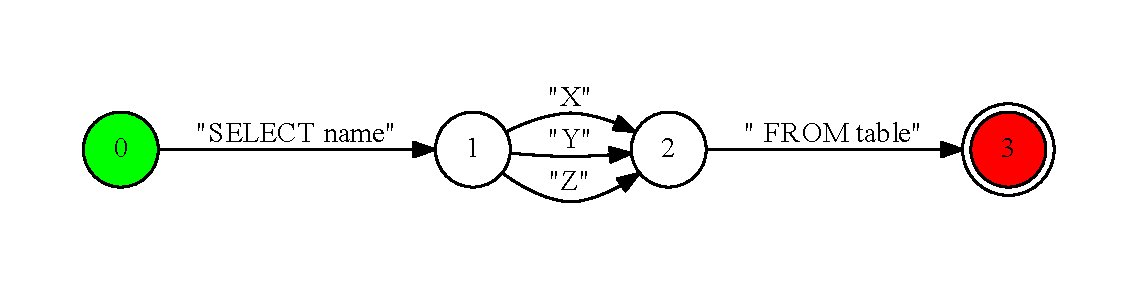
\includegraphics[width=1.0\linewidth]{tsql_test}}
\end{center}

\item Результат лексического анализа:
\begin{center}
    {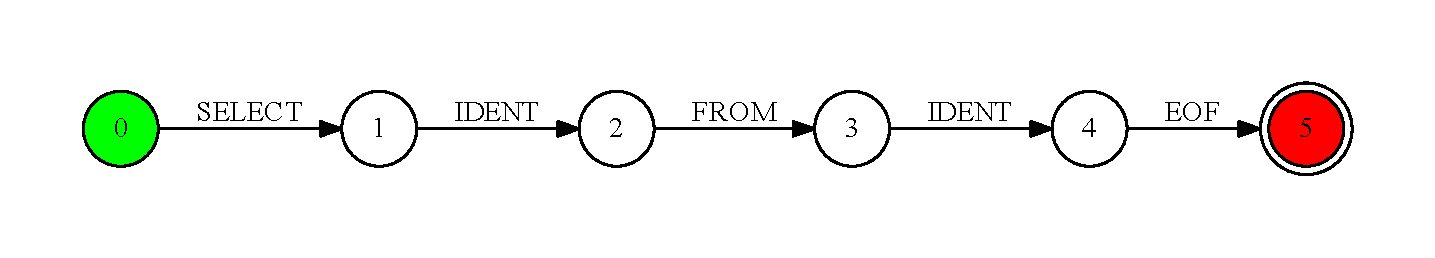
\includegraphics[width=1.0\linewidth]{tsql_test_appr}}
\end{center}
\end{itemize}
\end{frame}


\begin{frame}[fragile]
\transwipe[direction=90]
\frametitle{Пример}
\begin{itemize}
\item Результат лексического анализа:
	\begin{center}
        {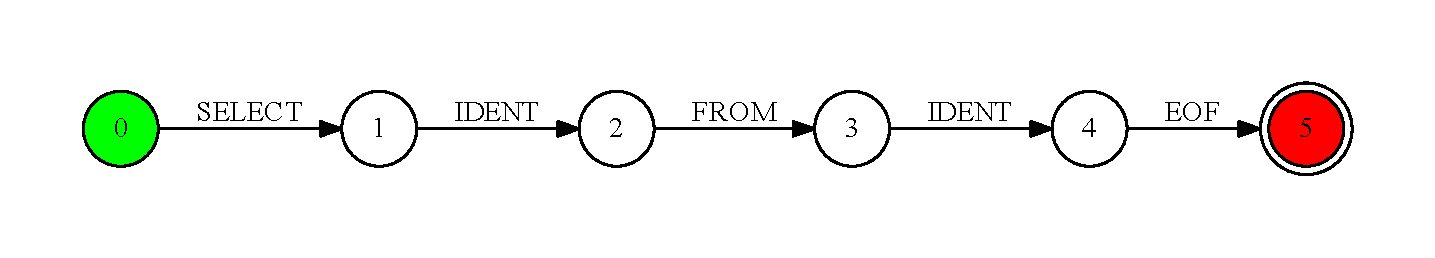
\includegraphics[width=1.0\linewidth]{tsql_test_appr}}
    \end{center}
		
\item Конечный автомат первого токена \verb|IDENT|:
	\begin{center}
        {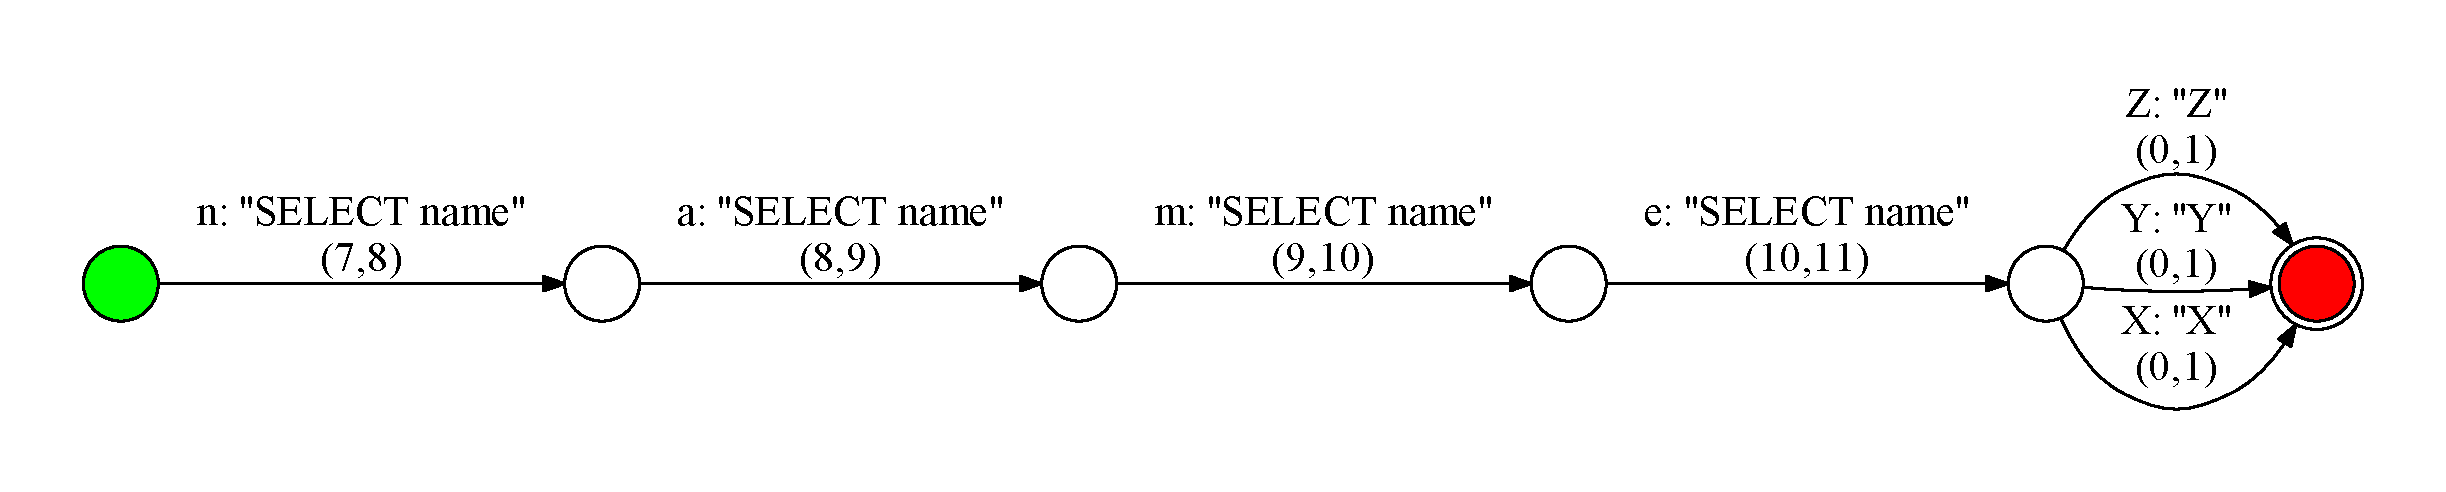
\includegraphics[width=1.0\linewidth]{tsql_ident_1}}
    \end{center}

\item Конечный автомат второго токена \verb|IDENT|:
	\begin{center}
        {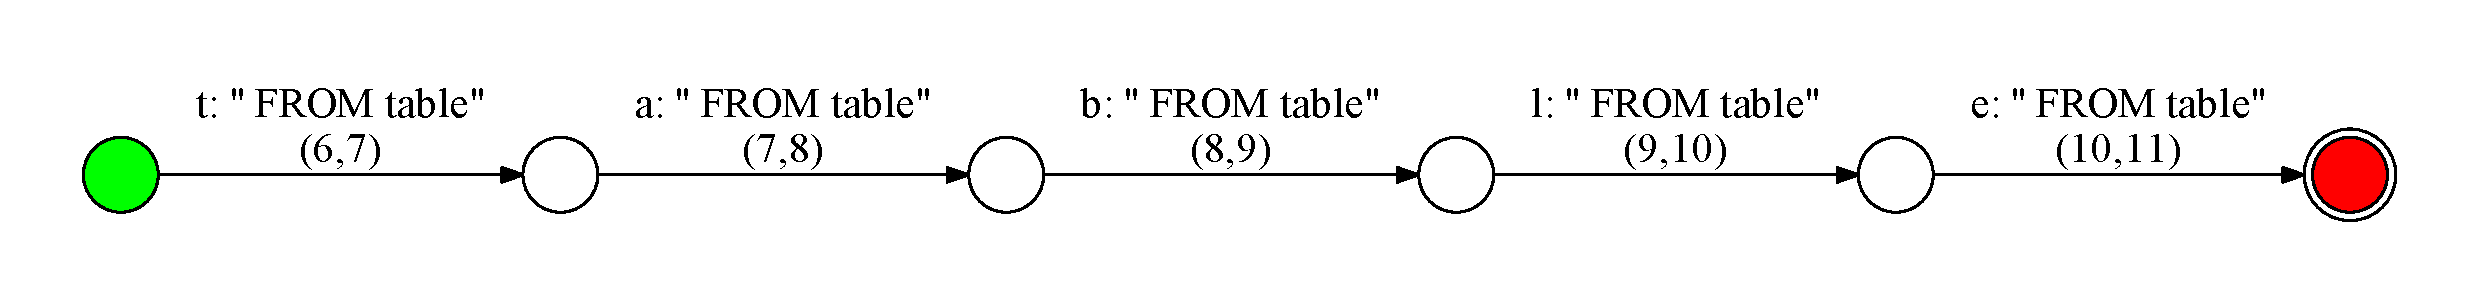
\includegraphics[width=1.0\linewidth]{tsql_ident_2}}
    \end{center}
\end{itemize}
\end{frame}


\begin{frame}[fragile]
\transwipe[direction=90]
\frametitle{Строковые операции}
\begin{itemize}	
\item 
	\begin{Verbatim}[commandchars=\\\{\}]
\textcolor{blue}{string} s = \textcolor{red}{"SELECT nameX FROM tableY"};
s = s.Replace(\textcolor{red}{"SELECT nameX"}, \textcolor{red}{"b"});
	\end{Verbatim}	

\item Многие строковые операции могут быть выражены через строковую операцию Replace, каждый аргумент которой является конечный автомат

\item Для обработки строковой операции \verb|Replace| использовался алгоритм, описанный в статье Fang Yu  ``Automata-based symbolic string analysis for vulnerability detection''
\end{itemize}
\end{frame}


\begin{frame}[fragile]
\transwipe[direction=90]
\frametitle{Пример}
$M$ = \verb|replace|($M_1, M_2, M_3$)

\begin{tabular}{c c}		
 	 \begin{minipage}{.6\textwidth} 
     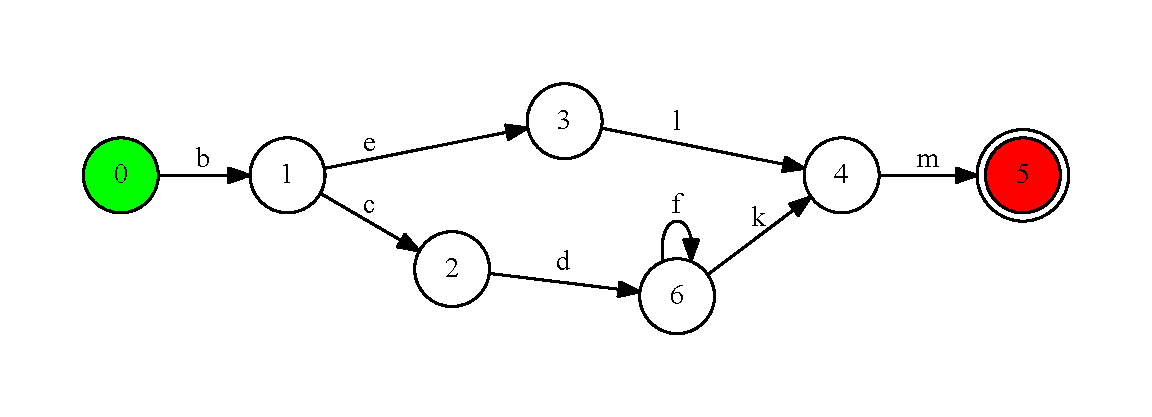
\includegraphics[width=\linewidth]{fsa1}
     \end{minipage} 
     &
 	 \begin{minipage}{.3\textwidth} 
     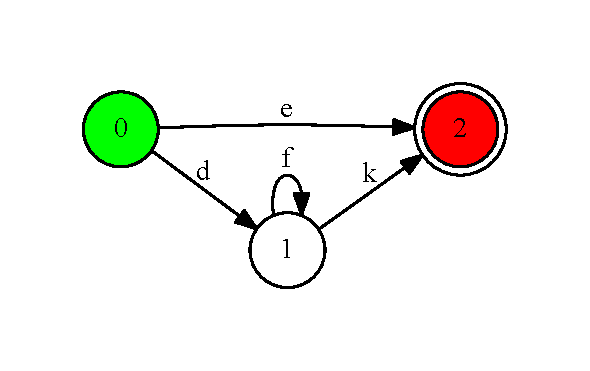
\includegraphics[width=\linewidth]{fsa2}
     \end{minipage} \\
     $M_1$ & $M_2$ \\
     \end{tabular}
     \begin{tabular}{c c}	
 	 \begin{minipage}{.25\textwidth} 
     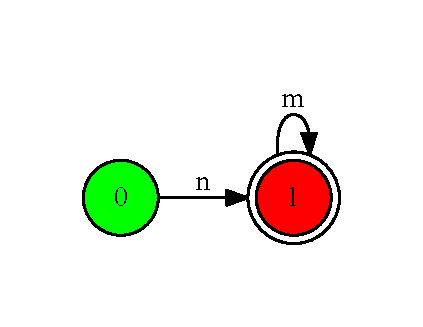
\includegraphics[width=\linewidth]{fsa3}
     \end{minipage} 
     &
 	 \begin{minipage}{.65\textwidth} 
     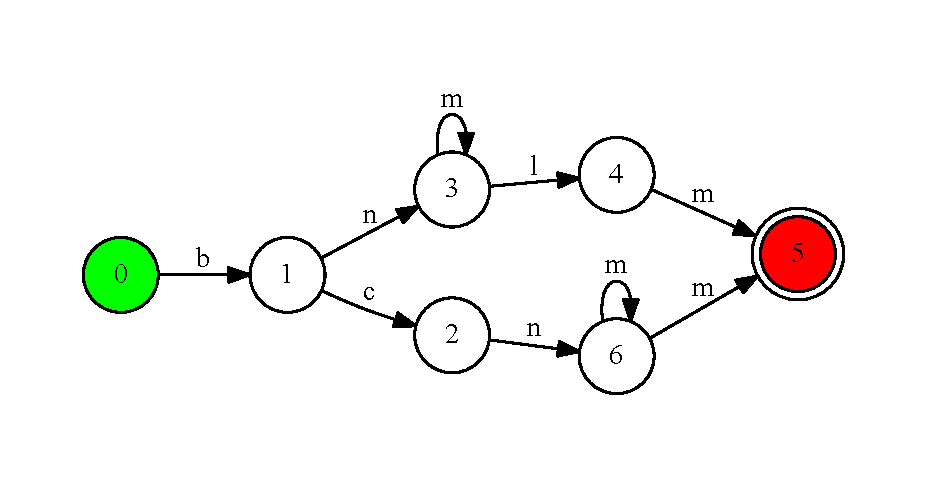
\includegraphics[width=\linewidth]{replace_example}
     \end{minipage} \\     
     $M_3$ & $M$ \\
\end{tabular}
\end{frame}

\begin{frame}[fragile]
\transwipe[direction=90]
\frametitle{Пример}

\begin{tabular}{c r}
     Входной граф: & Спецификация: \\
     \begin{minipage}{.4\textwidth} 
     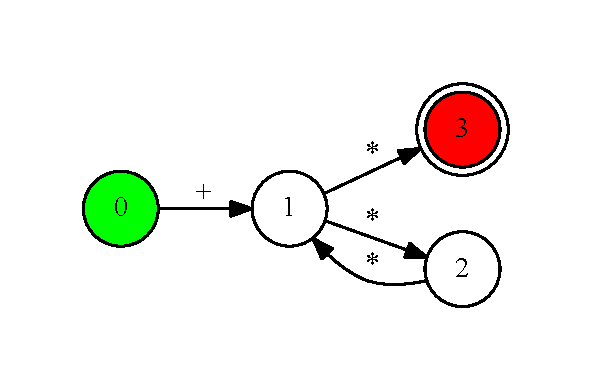
\includegraphics[width=\linewidth]{calc_ex}
     \end{minipage}  
     & 
	\begin{minipage}{.3\textwidth}    
	\begin{verbatim}
   PLUS : '+'
   POW : "**"
   MULT: '*'
	\end{verbatim}
	\end{minipage}
\end{tabular} 
 	
\begin{tabular}{l}		 	
	Результат лексического анализа: \\
    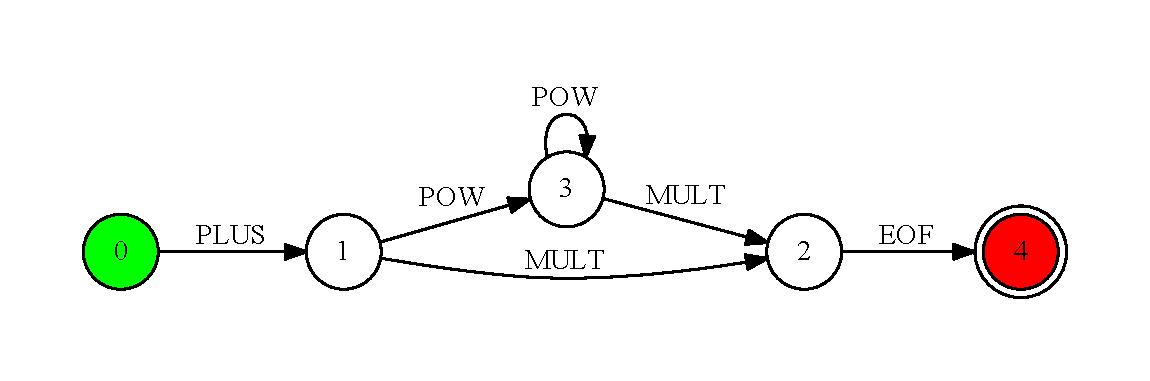
\includegraphics[width=0.8\linewidth]{calc_ex_res}    
\end{tabular}

\end{frame}

\begin{frame}
\transwipe[direction=90]
\frametitle{Инструмент YaccConstructor}
\begin{center}
	{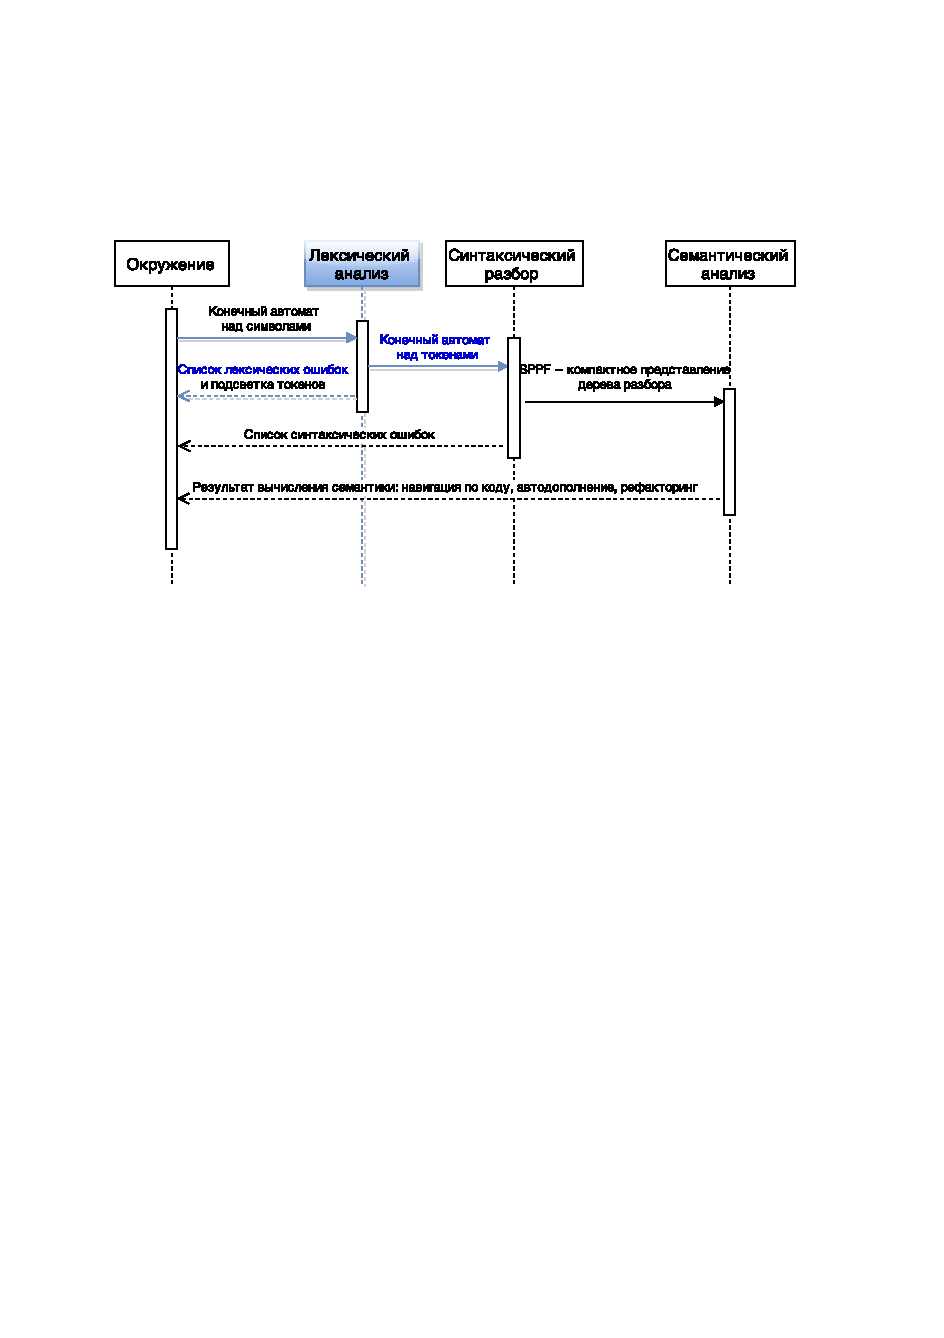
\includegraphics[width=1.0\linewidth]{Seq_with_lexer_highlighted_rus}}
\end{center}
\end{frame}


\begin{frame}
\transwipe[direction=90]
\frametitle{Архитектура инструмента}
\begin{center}
   {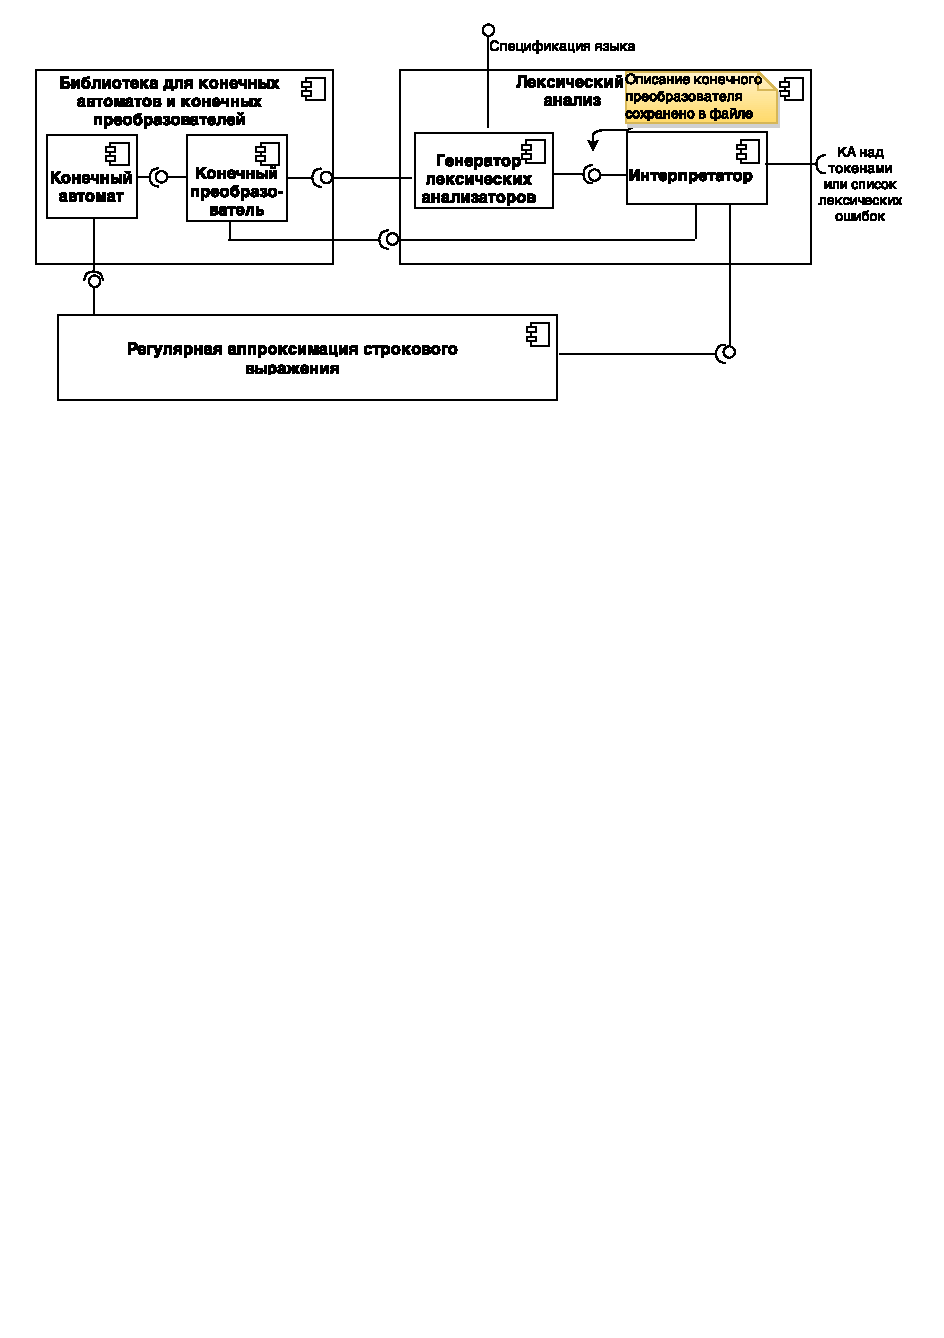
\includegraphics[width=1.0\linewidth]{ComponentDiagram_rus}}
\end{center}
\end{frame}


\begin{frame}%[t]
\transwipe[direction=90]
\frametitle{Результаты}

\begin{itemize}
\item Разработан алгоритм лексического анализа строковых выражений, формируемых с помощью циклов и строковых операций, сохраняющий привязку к исходному коду 
\item Реализована архитектура инструмента в рамках проекта YaccConstructor
\item Проведена апробация полученного инструмента
\item Результаты представлены на конференции CEE-SECR-2014
\item Публикация ``Инструментальная поддержка встроенных языков в интегрированных средах разработки'' (ВАК)
\end{itemize}
\end{frame}

\end{document}
